\documentclass[12pt]{article}
\usepackage{amsmath,amscd,amssymb}
\usepackage[pdftex]{graphicx}
\usepackage{array}
\usepackage{bbold}
\usepackage{amsfonts}  
\usepackage{bm}

\usepackage{tikz-qtree}
\usepackage{tikz}
\usetikzlibrary{bayesnet}
\usetikzlibrary{calc}

\begin{document}

%%% MODEL figure
\begin{figure}[t]	
	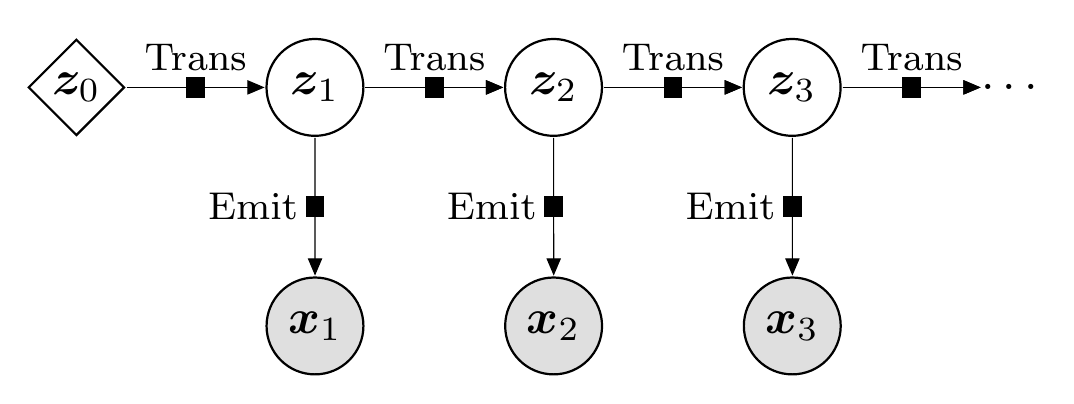
\begin{tikzpicture}[scale=1.75, transform shape,blackdot/.style={thin, draw=black, align=center, scale = 0.3,fill=black}]
    %\node [thick,det, left= of zhat1, xshift=5pt](zhat0) {$\bm{z}_0$};
    \node [thick, det] (z0) {$\bm{z}_0$};
    \node [thick, latent, right= of z0] (z1) {$\bm{z}_1$};
    \node [thick, latent, right= of z1] (z2) {$\bm{z}_2$};
    \node [thick, latent, right= of z2] (z3) {$\bm{z}_3$};
	\node [const, right=of z3] (dotsz) {\ldots};
    \node [thick, obs, below= of z1] (x1) {$\bm{x}_1$};
    \node [thick, obs, below= of z2] (x2) {$\bm{x}_2$};
    \node [thick, obs, below= of z3] (x3) {$\bm{x}_3$};
	\edge {z1} {z2};
	\edge {z2} {z3};
	\edge {z3} {dotsz};
    %\draw[->]  (z0) -- (z1);
    \draw[->]  (z0) -- node[blackdot] {d} node[above,font=\footnotesize] {Trans} (z1);
    \draw[->]  (z1) -- node[blackdot] {d} node[above,font=\footnotesize] {Trans} (z2);
    \draw[->]  (z1) -- node[blackdot] {d} node[left,font=\footnotesize] {Emit} (x1);
    \draw[->]  (z2) -- node[blackdot] {d} node[above,font=\footnotesize] {Trans} (z3);
    \draw[->]  (z2) -- node[blackdot] {d} node[left,font=\footnotesize] {Emit}(x2);
    \draw[->]  (z3) -- node[blackdot] {d} node[left,font=\footnotesize] {Emit}(x3);
    \draw[->]  (z3) -- node[blackdot] {d} node[above,font=\footnotesize] {Trans} (dotsz);
	\end{tikzpicture}\quad
\end{figure}	

\definecolor{lightblue}{RGB}{229, 236, 255}
\definecolor{darkblue}{RGB}{51, 133, 255}

%%% GUIDE figure
\begin{figure}[t]
	\begin{tikzpicture}[scale=1.5, transform shape]
	\tikzstyle{recnet}=[rectangle,fill=lightblue,draw=black,minimum size=17pt,inner sep=2pt]
    \node [thick,obs] (x1) {$\bm{x}_1$};
    \node [thick,obs, right= of x1, xshift=5pt] (x2) {$\bm{x}_2$};
    \node [thick,obs, right= of x2, xshift=5pt] (xT) {$\bm{x}_3$};
		
    \node [thick,det, above= of x1] (h1L) {$\bm{h}_1$};
    \node [thick,det, above= of x2] (h2L) {$\bm{h}_2$};
    \node [thick,det, above= of xT] (hTL) {$\bm{h}_3$};
	\node [const, left= of h1L, xshift=5pt](hRlabel){RNN};

	\node [thick, recnet, above= of h1L] (z1) {$(\mu_1, \sigma_1)$};
	\node [thick, recnet, above= of h2L] (z2) {$(\mu_2, \sigma_2)$};
	\node [thick, recnet, above= of hTL] (zT) {$(\mu_3, \sigma_3)$};
	\node [const, left=of z1, xshift=25pt](comb){{Combiners}};
	
	\node [const, above= of z1, yshift=-20pt, xshift=-33pt, darkblue](label1){};
	\node [const, above= of z2, yshift=-20pt, xshift=-33pt, darkblue](label2){};
	\node [const, above= of zT, yshift=-20pt, xshift=-33pt, darkblue](label3){};

	\node [thick,latent, above= of z1] (zhat1) {$\bm{z}_1$};
	\node [thick,latent, above= of z2] (zhat2) {$\bm{z}_2$};
	\node [thick,latent, above= of zT] (zhatT) {$\bm{z}_3$};
   	\node [thick,det, left= of zhat1, xshift=5pt](zhat0) {$\bm{z}_0^{\rm{q}}$};
	
	\edge [thick,red]{h2L} {h1L};	
	\edge [thick,red]{hTL}{h2L};	
	
	\edge [thick,red, bend left]{x1} {h1L};
	\edge [thick,red, bend left]{x2} {h2L};
	\edge [thick,red, bend left]{xT} {hTL};
	\edge [thick,darkblue]{h1L} {z1};
	\edge [thick,darkblue]{h2L} {z2};
	\edge [thick,darkblue]{hTL} {zT};
	\edge [thick]{z1}{zhat1};
	\edge [thick]{z2}{zhat2};
    \edge [thick]{zT}{zhatT};
    \edge [thick,darkblue,shorten <=0pt]{zhat0}{z1};
    \edge [thick,darkblue]{zhat1}{z2};
    \edge [thick,darkblue]{zhat2}{zT};
	\end{tikzpicture} 
\end{figure}

\end{document}
